\documentclass[12pt]{article}


% -------------------- PAQUETES --------------------
\usepackage[utf8]{inputenc}
\usepackage[spanish]{babel}
\usepackage[margin=2.54cm]{geometry}
\usepackage{graphicx}
\usepackage{xcolor}


% -------------------- CARGA DE ARCHIVOS EXTERNOS --------------------
% ----------------- UTILIDADES PARA DAR UN MEJOR FORMATO DE DOCUMENTO -----------------  


\definecolor{azul}{rgb}{0.0039, 0.3098, 0.6196}


% Formato para el indice general ...........
\makeatletter
    \renewcommand{\@dotsep}{1.5}
    \renewcommand{\l@section}{\@dottedtocline{1}{1.5em}{2.3em}}
    \renewcommand{\l@subsection}{\@dottedtocline{2}{3.8em}{3.2em}}
    \renewcommand{\l@subsubsection}{\@dottedtocline{3}{7.0em}{4.1em}}
\makeatother

% --------- COMANDOS PERSONALIZADOS PARA LA PORTADA DE LAS TAREAS, TRABAJOS Y PROYECTOS ---------

\newcommand{\rutaLogo}[1]{\newcommand{\RutaLogo}{#1}}
\newcommand{\tema}[1]{\newcommand{\Tema}{#1}}
\newcommand{\etiquetaAutores}[1]{\newcommand{\EtiquetaAutores}{#1}}
\newcommand{\alumno}[1]{\newcommand{\Alumno}{#1}}
\newcommand{\materia}[1]{\newcommand{\Materia}{#1}}
\newcommand{\docente}[1]{\newcommand{\Docente}{#1}}
\newcommand{\ciclo}[1]{\newcommand{\Ciclo}{#1}}
\newcommand{\fecha}[1]{\newcommand{\Fecha}{#1}}
\newcommand{\periodo}[1]{\newcommand{\Periodo}{#1}}



% -------------------- DEFINICIÓN DE LA PORTADA --------------------
\rutaLogo{../../../RecursosGlobales/Img/logo_tec_azuay.png}
\tema{\\ \vspace{1cm} Actividad N°4: Tablas de verdad \\ \vspace{1.7cm}}
\etiquetaAutores{Alumno:}
\alumno{Eduardo Mendieta \vspace{1cm}}
\materia{Matemática \vspace{1cm}}
\docente{Lcda. Vilma Duchi \vspace{1cm}}
\ciclo{Primer Ciclo \vspace{1.1cm}}
\fecha{10 de junio de 2024 \vspace{1cm}}
\periodo{Abril 2024 - Agosto 2024}



% -------------------- INFORME --------------------
\begin{document}

    \begin{titlepage}

    \centering

    \includegraphics[width=0.11\textwidth]{\RutaLogo} 

    \vspace{0.3cm}
    \textcolor{azul}{\Large \textbf{Instituto Superior Universitario Tecnológico del Azuay \\}}
    \vspace{0.3cm}
    \textcolor{azul}{\Large \textbf{Tecnología Superior en Big Data}}
    
    % 1. ---------------- TEMA -------------------------
    
    {\Large\textbf{\Tema}}
    
    % 2. ---------------- AUTOR(ES) -------------------------
    \textcolor{azul}{\large \textbf{\EtiquetaAutores} \\}
    \vspace{0.3cm}
    {\large \Alumno}

    % 3. ---------------- MATERIA -------------------------
    \textcolor{azul}{\large \textbf{Materia:} \\}
    \vspace{0.3cm}
    {\large \Materia}


    % 3. ---------------- DOCENTE -------------------------
    \textcolor{azul}{\large \textbf{Docente:} \\}
    \vspace{0.3cm}
    {\large \Docente}


    % 3. ---------------- Ciclo -------------------------
    \textcolor{azul}{\large \textbf{Ciclo:} \\}
    \vspace{0.3cm}
    {\large \Ciclo}


    % 3. ---------------- FECHA -------------------------
    \textcolor{azul}{\large \textbf{Fecha:} \\}
    \vspace{0.3cm}
    {\large \Fecha}

    % 3. ---------------- PERIODO -------------------------
    \textcolor{azul}{\large \textbf{Periodo Académico:} \\}
    \vspace{0.3cm}
    {\large \Periodo}
 
\end{titlepage}

  
    \section*{\centering Actividad N°4: Tablas de verdad}
        \textbf{Formaliza los siguientes argumentos y halla la tabla de verdad:}

        \begin{enumerate}
             % EJERCICIO 1: ----------------------------------------------------
            \item \textbf{Aprobare lógica, si Dios quiere. Aprobare lógica si y sólo si estudio y hago todos los ejercicios. Sin embargo, no he hecho los ejercicios, así que Dios no quiere que apruebe lógica.}
                \par$p:$ Aprobaré lógica.
                \par$q:$ Si Dios quiere.
                \par$r:$ Estudio.
                \par$s:$ Hago todos los ejercicios.
                \par$n = 4$, $2^n = 2^4 = 16$
                \par\vspace{0.5cm}$[(p \longrightarrow q) \wedge (p \longleftrightarrow (r \wedge s)) \wedge \sim s] \longrightarrow (\sim q \longrightarrow \sim p)$ 
            
                \begin{figure}[!h]
                    \centering
                    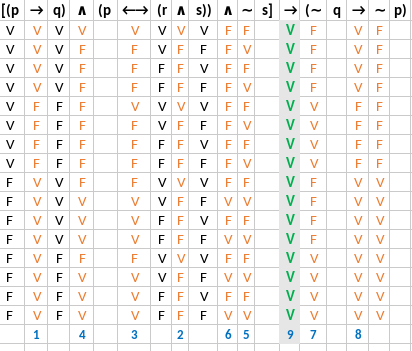
\includegraphics[width=0.6\textwidth]{Img/Tarea4_ej1.png}
                \end{figure}

                \textbf{Respuesta:} El enunciado es una tautología.

                % EJERCICIO 2: ----------------------------------------------------
                \newpage
                \item \textbf{Si la tormeta continúa o anochece, nos quedaremos a cenar o a dormir. Si nos quedamos a cenar o a dormir, no iremos mañana al concierto. Pero si iremos mañana al concierto. Así pues, la tormenta no continúa.}
                \par$p:$ La tormenta continúa.
                \par$q:$ Anochece.
                \par$r:$ Nos quedaremos a cenar.
                \par$s:$ Nos quedamos a dormir.
                \par$t:$ Iremos mañana al concierto.
                \par$n = 5$, $2^n = 2^5 = 32$
                \par\vspace{0.5cm}$[(p \vee q) \longrightarrow (r \vee s)] \wedge [(r \vee s) \longrightarrow \sim t] \wedge (t \longrightarrow \sim p)$
            
                \begin{figure}[!h]
                    \centering
                    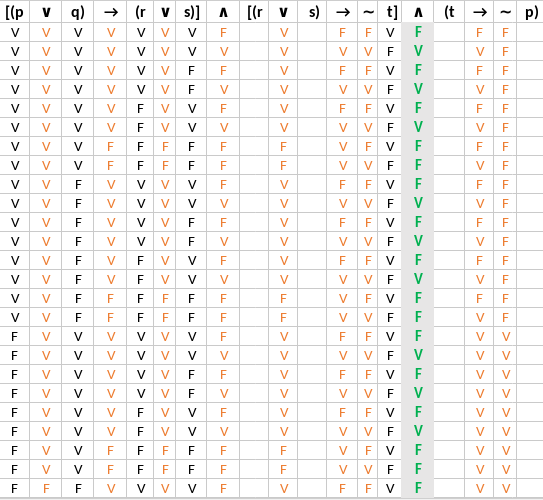
\includegraphics[width=0.6\textwidth]{Img/Tarea4_ej2_1.png}
                \end{figure}

                \begin{figure}[!h]
                    \centering
                    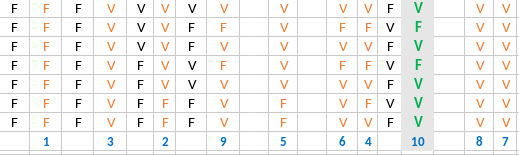
\includegraphics[width=0.6\textwidth]{Img/Tarea4_ej2_2.png}
                \end{figure}

                \textbf{Respuesta:} El enunciado es una contingencia.

             % EJERCICIO 3: ----------------------------------------------------
             \newpage
            \item \textbf{Si no es cierto que se puede ser rico y dichoso a la vez, entonces la vida está llena de frustraciones y no es un camino de rosas. Si se es feliz, no se puede tener todo. Por consiguiente, la vida está llena de frustraciones.}
                \par$p:$ Se puede ser rico.
                \par$q:$ Se puede ser dichoso.
                \par$r:$ La vida está llena de frustraciones.
                \par$s:$ Es un camino de rosas.
                \par$n = 4$, $2^n = 2^4 = 16$
                \par\vspace{0.5cm}$[(\sim (p \wedge q) \longrightarrow (r \wedge \sim s)) \wedge (q \longrightarrow \sim p)] \longrightarrow r$
             
                \begin{figure}[!h]
                    \centering
                    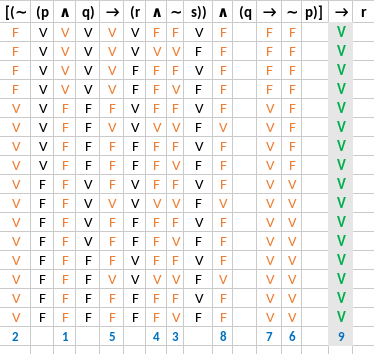
\includegraphics[width=0.6\textwidth]{Img/Tarea4_ej3.png}
                \end{figure}

                \textbf{Respuesta:} El enunciado es una tautología.
                % EJERCICIO 4: ----------------------------------------------------
             \newpage
            \item \textbf{La vida no tiene cosas así de fuertes o yo te puedo contar cómo es una llama por dentro. Si yo te puedo contar cómo es una llama por dentro, entonces pienso entregarte mi tiempo y pienso entregarte mi fe. No es cierto que piense entregarte mi tiempo y piense entregarte mi fe. Por lo tanto, la vida no tiene cosas así de fuertes.}
                \par$p:$ La vida tiene cosas asi de fuertes.
                \par$q:$ Te puedo contar cómo es una llama por dentro.
                \par$r:$ Pienso entregarte mi tiempo.
                \par$s:$ Pienso entregarte mi fe.
                \par$n = 4$, $2^n = 2^4 = 16$
                \par\vspace{0.5cm}$[(\sim p \vee q) \wedge (q \longrightarrow (r \wedge s)) \wedge (\sim (r \wedge s))] \longrightarrow \sim p$
                
                \begin{figure}[!h]
                    \centering
                    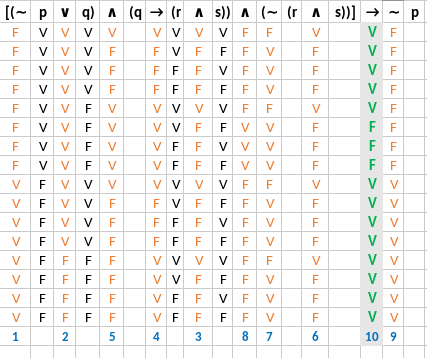
\includegraphics[width=0.6\textwidth]{Img/Tarea4_ej4.png}
                \end{figure}

                \textbf{Respuesta:} El enunciado es una contingencia.

        \end{enumerate}

\end{document}